Il presente capitolo illustra l'analisi dei requisiti e la progettazione architetturale del sistema. La struttura del capitolo segue un approccio incrementale: si definiscono i requisiti operativi, si progetta l'infrastruttura Cloud di base (strategia Multi-Account e Serverless), si modella il livello di persistenza e i flussi dati (Event-Driven, S3, DynamoDB) e si definisce l'architettura interna del software applicativo. Infine, vengono delineati i processi di automazione e le pratiche di Infrastructure as Code necessari a governare il ciclo di vita del software. L'obiettivo è fornire una giustificazione formale e ingegneristica per ogni scelta tecnologica, ponendo le basi per l'implementazione descritta nel capitolo successivo.

\section{Analisi del Contesto Operativo e Definizione dei Requisiti}
\label{sec:analisi_contesto}

L'analisi del contesto operativo esamina le criticità intrinseche alle infrastrutture tradizionali impiegate nel settore dell'advertising digitale. Questo dominio applicativo impone l'elaborazione di elevati volumi di dati in tempo reale e richiede la gestione di carichi di rete altamente variabili. L'ispezione delle architetture legacy evidenzia limitazioni strutturali derivanti dall'eterogeneità dei servizi e dall'esecuzione parzialmente manuale delle procedure di rilascio. L'assenza di un sistema di versionamento dichiarativo impedisce la tracciabilità delle modifiche infrastrutturali e compromette la riproducibilità degli ambienti operativi. Tale debito tecnico costringe i sistemi a un'allocazione statica delle risorse computazionali, la quale risulta indipendente dal carico effettivo e incapace di adattarsi dinamicamente alle fluttuazioni del traffico.

L'identificazione di questi colli di bottiglia operativi determina la formulazione di tre requisiti architetturali primari per la progettazione del nuovo sistema Cloud-Native.

Il primo requisito definisce la necessità di una scalabilità elastica. L'architettura deve allocare e deallocare dinamicamente le risorse computazionali per assorbire i picchi di traffico imprevisti. Questa elasticità deve garantire latenze di elaborazione minime senza richiedere alcun intervento di ridimensionamento manuale da parte di un operatore.

Il secondo vincolo architetturale impone l'isolamento degli ambienti operativi. Il sistema deve garantire una separazione logica e fisica rigorosa tra le risorse destinate alla programmazione, alle fasi di collaudo e all'ambiente di produzione. Tale segregazione previene interferenze tra i carichi di lavoro e assicura che i test non impattino le prestazioni dei servizi esposti agli utenti finali.

Infine, il terzo requisito prescrive la tracciabilità e l'automazione integrale dei flussi operativi. La progettazione deve vincolare la gestione dei componenti cloud all'utilizzo di codice dichiarativo, trattando l'infrastruttura alla stregua del software applicativo. Parallelamente, il sistema deve implementare pipeline automatizzate per disciplinare i processi di integrazione e di rilascio continuo (CI/CD), eliminando le operazioni manuali.

\section{Progettazione dell'Infrastruttura Cloud}
\label{sec:design_infrastruttura}

Per soddisfare i requisiti prestazionali, l'architettura si basa sul paradigma Serverless \cite{BerkeleyServerless}, implementato tramite Amazon Web Services (AWS). Questa scelta rimuove l'onere della gestione di macchine virtuali e introduce un modello di costo calcolato sui tempi di esecuzione effettivi.

Come illustrato nello schema logico in Figura \ref{fig:architettura_serverless_overview}, per garantire la modularità l'architettura è stata concettualmente divisa in due categorie funzionali: i servizi di backend (Services), deputati all'esposizione di interfacce di programmazione sincrone, e i componenti asincroni (Workers), dedicati all'elaborazione in background dei dati.

\begin{figure}[htbp]
    \centering
    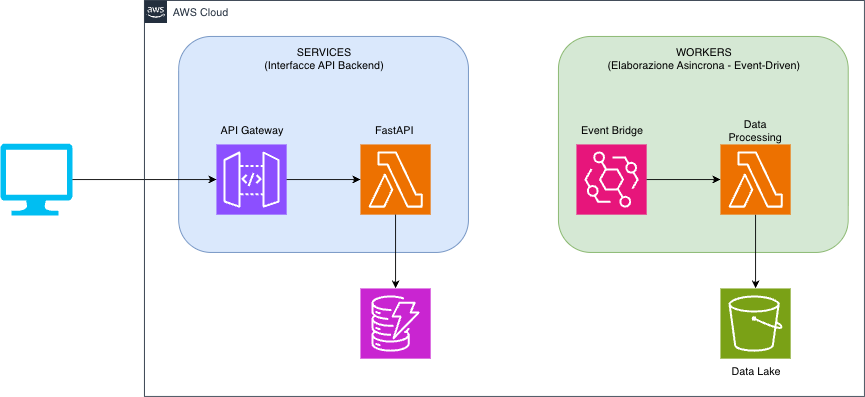
\includegraphics[width=1\textwidth]{images/services_workers.drawio.png}
    \caption{Schema concettuale dell'architettura Serverless su AWS, illustrante la separazione tra Services (interfacce sincrone) e Workers (elaborazione asincrona) [Elaborazione dell'autore].}
    \label{fig:architettura_serverless_overview}
\end{figure}

\subsection{Strategia Multi-Account e Segregazione delle Risorse}

L'impiego di un singolo account AWS per l'intero ciclo di vita del software estende pericolosamente il dominio di faglia in caso di incidenti e complica il controllo degli accessi. La progettazione ha quindi previsto una strategia Multi-Account, la cui topologia è rappresentata in Figura \ref{fig:aws_multi_account_topology}, strutturata su tre ambienti isolati: Sviluppo (Dev), Produzione (Prod) e Condiviso (Shared).

Gli account Dev e Prod sono copie speculari, garantendo che le configurazioni validate in sviluppo si comportino in modo deterministico in produzione. L'account Shared agisce come nodo centralizzato, ospitando le risorse accessibili trasversalmente: i registri Amazon ECR \cite{ECR} per le immagini Docker e i bucket S3 per gli artefatti statici. Questa topologia centralizzata previene la duplicazione dei pacchetti e permette ai flussi di deployment di prelevare gli artefatti da un'unica sorgente sicura.

\begin{figure}[htbp]
    \centering
    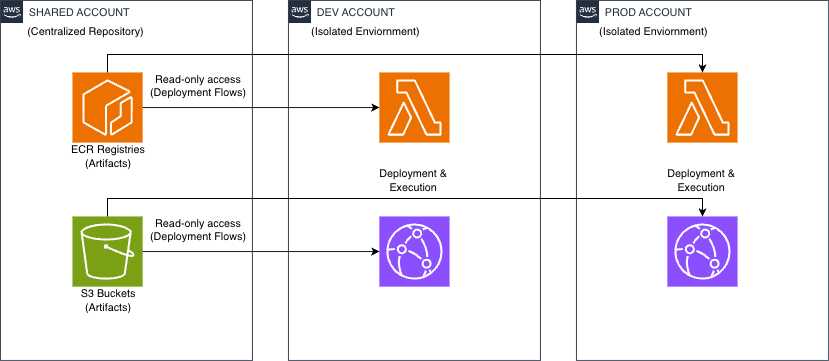
\includegraphics[width=0.95\textwidth]{images/aws-multi-account.drawio.png}
    \caption{Topologia della strategia Multi-Account su AWS. L'account Shared centralizza gli artefatti, referenziati in sola lettura per il deployment negli ambienti isolati [Elaborazione dell'autore].}
    \label{fig:aws_multi_account_topology}
\end{figure}

\section{Progettazione del Livello Dati e Flussi Asincroni}
\label{sec:design_dati}

L'architettura separa le responsabilità tra l'archiviazione di volumi massivi per l'analisi e la memorizzazione transazionale a bassa latenza, introducendo un netto disaccoppiamento tra produttori e consumatori di dati.

\subsection{Decomposizione Event-Driven ed ETL Serverless}

I processi di elaborazione dati sono stati re-ingegnerizzati applicando il pattern Event-Driven \cite{EventDrivenArchitecture}. I flussi di estrazione e trasformazione (ETL) sono composti da microservizi specializzati asincroni.
Come delineato in Figura \ref{fig:pipeline-etl}, i servizi di estrazione depositano i dati grezzi in un Data Lake su Amazon S3 \cite{S3Doc}. L'inserimento di un file innesca automaticamente l'esecuzione di funzioni AWS Lambda \cite{AWSLambdaDoc} o processi AWS Glue \cite{AWSGlueDoc}. Questi componenti applicano le regole di pulizia e salvano i dati nel formato colonnare Parquet.

\begin{figure}[ht!]
    \centering
    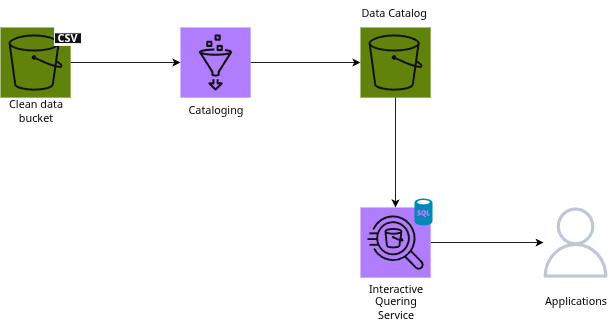
\includegraphics[width=1\textwidth]{images/elaborazione-serverless.drawio.png}
    \caption{Pipeline di elaborazione dati Serverless. AWS Glue trasforma i dati grezzi su S3 rendendoli interrogabili tramite Athena [Elaborazione dell'autore].}
    \label{fig:pipeline-etl}
\end{figure}

\subsection{Partizionamento Hive-Style del Data Lake}

Per ottimizzare le prestazioni e mitigare i costi operativi, il Data Lake è diviso in due zone logiche distinte: Raw (per i dati estratti nel formato originale) e Clean (per i dati trasformati e standardizzati). I dati immagazzinati nella zona Clean sono archiviati applicando rigorosamente un partizionamento Hive-style \cite{HiveStyle}. Questo paradigma organizza i file in percorsi gerarchici auto-descrittivi basati su coordinate temporali, ad esempio, \texttt{anno=2024/mese=10/giorno=25/}, come visualizzato nella gerarchia di Figura \ref{fig:s3_hive_partitioning}.

\begin{figure}[htbp]
    \centering
    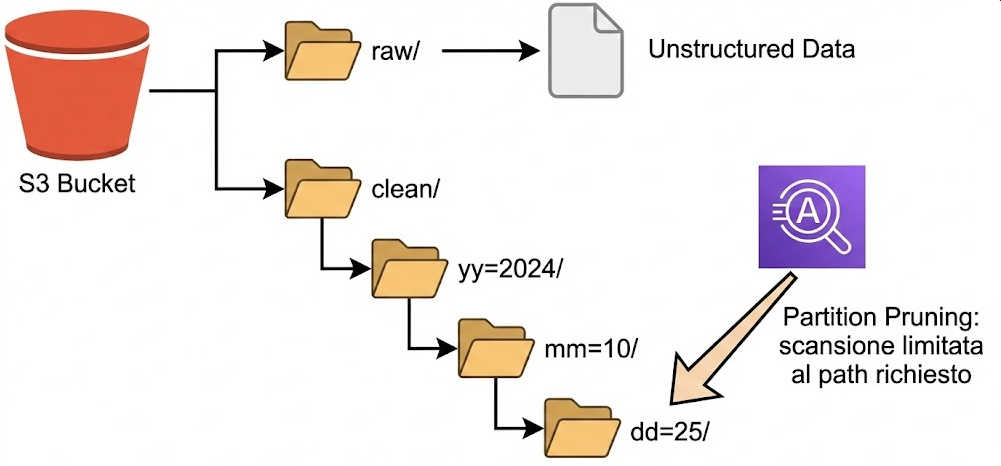
\includegraphics[width=1\textwidth]{images/partition-pruning.png}
    \caption{Struttura gerarchica del Data Lake su Amazon S3 basata su partizionamento Hive-style. L'organizzazione abilita il partition pruning da parte di Amazon Athena [Elaborazione dell'autore].}
    \label{fig:s3_hive_partitioning}
\end{figure}

Questo design logico permette ad Amazon Athena \cite{Athena} di eseguire l'operazione di partition pruning, ignorando sistematicamente le directory non pertinenti alla query SQL in esecuzione. Per quantificare l'impatto architetturale di tale scelta, si consideri l'esecuzione di un'interrogazione analitica tipica per l'estrazione delle metriche giornaliere relative a una specifica campagna pubblicitaria:

\begin{lstlisting}[language=SQL]
SELECT campaign_id, SUM(impressions) AS total_impressions
FROM impressions_table
WHERE campaign_id = 'ABC-123' 
  AND year = '2024' AND month = '10' AND day = '25';
\end{lstlisting}

In un Data Lake privo di partizionamento logico, il motore di query distribuito è costretto a leggere sequenzialmente l'intero volume di dati archiviato nel bucket Amazon S3 per individuare i record. Assumendo un volume di 1 Terabyte (TB) di dati storici, l'operazione comporta la scansione dell'intero Terabyte, incorrendo nel costo fisso per TB associato ad Athena.

Sfruttando il partizionamento, il motore interroga preventivamente il catalogo dati per risolvere i predicati della clausola WHERE associati alle chiavi di partizione. Questa operazione permette ad Athena di accedere esclusivamente al prefisso S3 isolato. Se il volume di dati generato nella singola giornata ammonta a 10 Gigabyte (GB), il sistema scansiona esclusivamente tale frazione, traducendosi in una riduzione del 99\% dei dati elaborati, con un conseguente abbattimento dei costi e della latenza.

\subsection{Modellazione NoSQL: Single Table Design}

La persistenza dello stato transazionale dei microservizi è demandata ad Amazon DynamoDB \cite{DynamoDBPaper}. La progettazione adotta massicciamente il Single Table Design \cite{SingleTableDesign}, memorizzando entità eterogenee all'interno di un'unica tabella, come esemplificato in Figura \ref{fig:single-table-design}. Sfruttando chiavi primarie composite (Partition Key e Sort Key) progettate ad hoc, il sistema recupera relazioni complesse con una singola operazione di lettura, minimizzando il consumo di Read Capacity Units (RCU).

\begin{figure}[ht!]
    \centering
    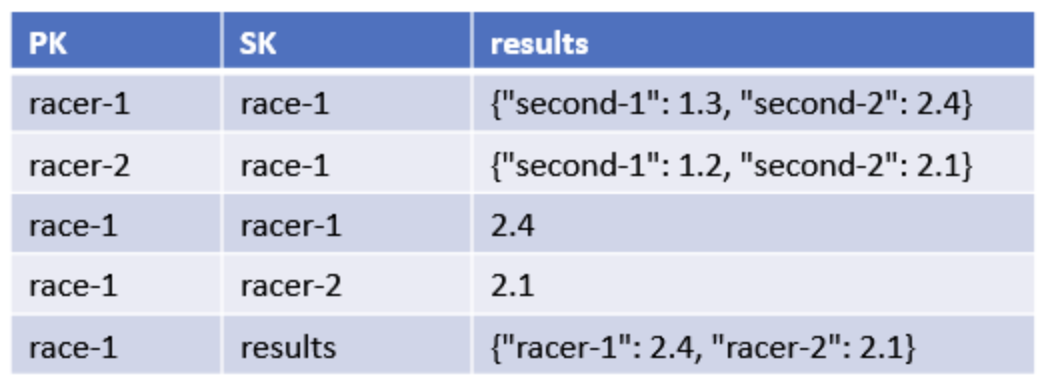
\includegraphics[width=1\textwidth]{images/single-table-design.png}
    \caption{Esempio di Single Table Design per la memorizzazione di entità eterogenee in una singola tabella \cite{SingleTableDesign}.}
    \label{fig:single-table-design}
\end{figure}

\section{Progettazione dei Servizi Applicativi}
\label{sec:design_backend}

I microservizi che espongono API sincrone richiedono un rigore strutturale per garantire la manutenibilità del codice e la stabilità delle interfacce pubbliche.

\subsection{Framework API e Validazione dei Dati}
\label{subsec:framework_fastapi}

Per lo sviluppo dei microservizi è stato selezionato il framework Python FastAPI \cite{FastAPIDoc}. In questo contesto, la libreria Pydantic assume un ruolo centrale per l'ispezione statica dei tipi e la validazione a runtime. Ogni payload JSON deve superare una convalida formale contro schemi predefiniti.

L'implementazione di questo meccanismo si fonda sulla definizione di Data Transfer Object (DTO). Di seguito è illustrato un modello rappresentativo per l'accettazione di un payload relativo a una campagna pubblicitaria:

\begin{lstlisting}[language=python]
from pydantic import BaseModel, Field, HttpUrl
from datetime import date

class CampaignCreateDTO(BaseModel):
    campaign_name: str = Field(..., min_length=3, max_length=100)
    budget: float = Field(..., gt=0)
    target_url: HttpUrl
    start_date: date
\end{lstlisting}

Quando il microservizio riceve una richiesta HTTP POST, il framework esegue la conversione automatica dei tipi e la validazione dei vincoli dichiarativi. Qualora il payload non rispetti i vincoli, ad esempio un budget negativo, l'istanza dell'oggetto non viene creata e la logica di business non viene invocata. Il framework genera in automatico una risposta HTTP 422, fornendo un corpo JSON che localizza l'errore:

\begin{lstlisting}
{
  "detail": [
    {
      "loc": ["body", "budget"],
      "msg": "Input should be greater than 0",
      "type": "greater_than",
      "ctx": {"gt": 0}
    }
  ]
}
\end{lstlisting}

Questa tipologia di validazione minimizza la necessità di scrivere codice procedurale per la gestione delle eccezioni.

\subsection{Architettura Interna: Clean Architecture e Dependency Injection}

Per prevenire un elevato accoppiamento strutturale, la base di codice aderisce ai principi della Clean Architecture \cite{CleanArchitecture}. Come mostrato in Figura \ref{fig:clean_architecture_fastapi}, il software è stratificato in tre livelli funzionali.

\begin{figure}[htbp]
    \centering
    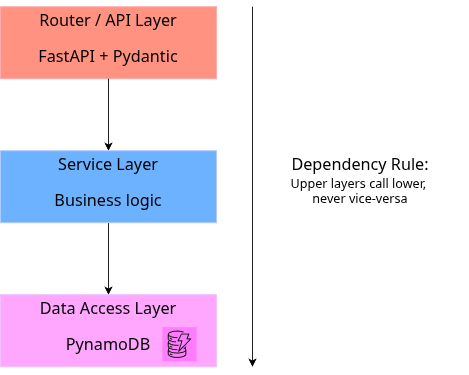
\includegraphics[width=1\textwidth]{images/clean-architecture.drawio.png}
    \caption{Stratificazione interna dei microservizi secondo i principi della Clean Architecture. Il flusso di controllo è unidirezionale dal livello di presentazione verso il livello di accesso ai dati [Elaborazione dell'autore].}
    \label{fig:clean_architecture_fastapi}
\end{figure}

Il primo strato è il Router Layer, che gestisce esclusivamente il routing HTTP. Il secondo è il Service Layer, contenente la logica di business agnostica rispetto a database e framework web. Il terzo è il Repository Layer, che incapsula le interazioni con S3 e DynamoDB.
Il passaggio di informazioni e dipendenze tra i livelli sfrutta il pattern Dependency Injection. Oltre all'iniezione delle dipendenze strutturali, il meccanismo è impiegato per le validazioni di dominio preliminari, permettendo ai controller di rimanere snelli.

\section{Osservabilità e Gestione delle Anomalie}
\label{sec:design_observability}

In ambienti Serverless distribuiti, l'assenza di server fisici impone l'adozione di meccanismi di tracciamento centralizzati e proattivi. Tutti i microservizi implementano un logger egualmente configurato che produce output in formato JSON strutturato, incanalato in Amazon CloudWatch. 

Per la gestione degli errori nei flussi asincroni, il design prevede l'utilizzo di Dead Letter Queue (DLQ), come illustrato in Figura \ref{fig:observability_dlq_flow}. I messaggi non elaborabili, dopo aver esaurito la politica di retry, vengono isolati in questa coda. L'evento di inserimento innesca notifiche tramite EventBridge \cite{EventBridgeDoc} verso i canali operativi aziendali, minimizzando i tempi di rilevamento.

\begin{figure}[htbp]
    \centering
    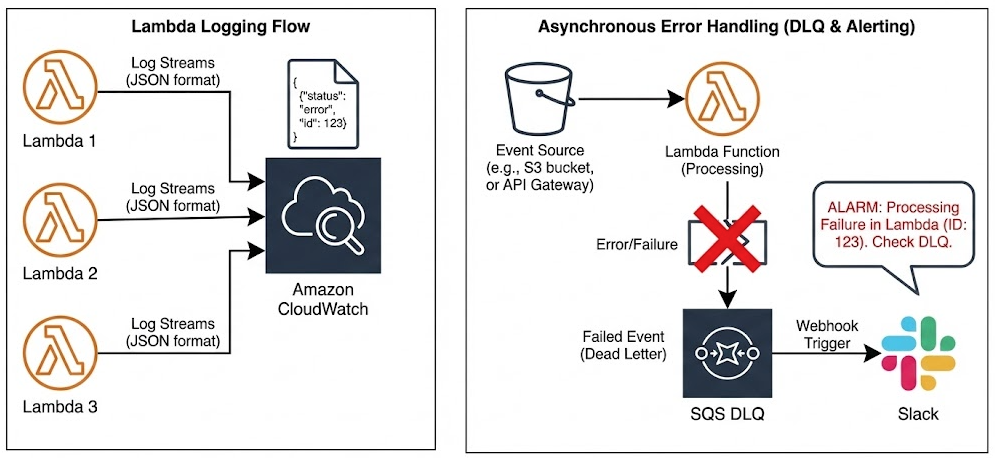
\includegraphics[width=1\textwidth]{images/dlq-logging.png}
    \caption{Flusso architetturale della telemetria. I log strutturati confluiscono in Amazon CloudWatch; i messaggi non processabili vengono isolati in una Dead Letter Queue (DLQ) innescando sistemi di notifica [Elaborazione dell'autore].}
    \label{fig:observability_dlq_flow}
\end{figure}

\section{Automazione e Infrastructure as Code (IaC)}
\label{sec:design_automazione}

La garanzia di riproducibilità è assicurata dalla traduzione dell'intera infrastruttura in codice dichiarativo e dall'automazione delle pipeline di rilascio.

\subsection{Topologia Architetturale del Codice IaC}

Le risorse cloud sono modellate tramite Terraform \cite{IaCGuerriero, TerraformUpAndRunning}. Per agevolare la governance, la progettazione adotta un singolo repository infrastrutturale centralizzato. Tuttavia, la gestione di un'infrastruttura di livello enterprise tramite un singolo file di stato (state file) monolitico costituisce un anti-pattern ingegneristico. Un file di stato di grandi dimensioni dilata i tempi di calcolo del grafo delle dipendenze e amplifica il raggio di impatto (blast radius) in caso di corruzione accidentale dello stesso.

Per mitigare tali criticità, la topologia del repository implementa un'architettura a strati, come schematizzato nella Figura \ref{fig:iac_terraform_workflow}. Il design impone una netta segregazione logica tra la definizione astratta delle risorse e la loro effettiva istanziazione negli ambienti cloud di destinazione.

\begin{figure}[htbp]
\centering
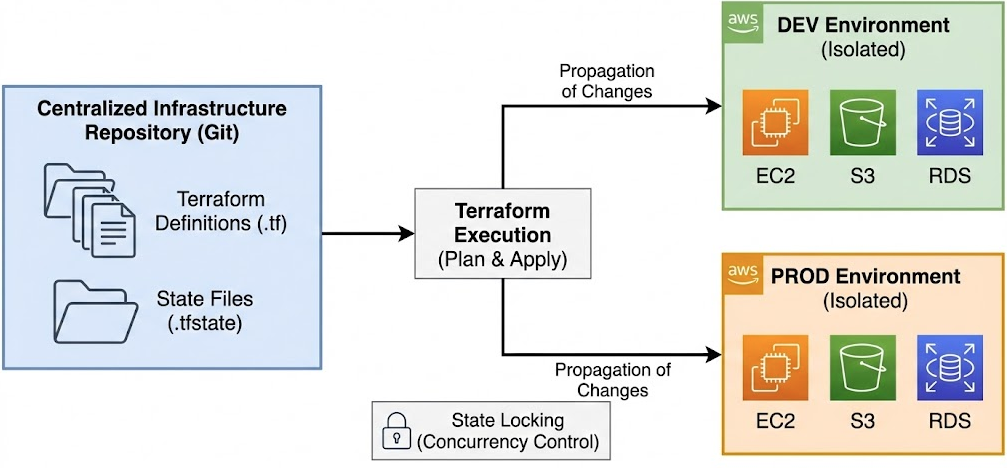
\includegraphics[width=1\textwidth]{images/flusso_iac.png}
\caption{Flusso di lavoro Infrastructure as Code: versionamento dello stato dichiarativo e propagazione delle modifiche tramite Terraform [Elaborazione dell'autore].}
\label{fig:iac_terraform_workflow}
\end{figure}

Il primo livello di questa astrazione è costituito dai moduli riutilizzabili. Ogni modulo incapsula i dettagli implementativi di un dominio architetturale specifico, come il provisioning di un cluster containerizzato o la configurazione di un database, ed espone esclusivamente un'interfaccia controllata di variabili in ingresso. Questo approccio garantisce che la logica di creazione delle risorse venga scritta e sottoposta a revisione una singola volta.

Per governare la topologia a strati e garantire il rispetto del principio DRY (\textit{Don't Repeat Yourself}), la progettazione architetturale prescrive l'adozione dell'orchestratore Terragrunt. Il livello di istanziazione (definito \textit{Live Environment}) delega a questo strumento la mappatura della topologia degli account AWS isolati (\texttt{dev}, \texttt{prod} e \texttt{shared}). Al fine di prevenire derive di configurazione (\textit{configuration drift}) tra i diversi ambienti, il design centralizza le definizioni, evitando la duplicazione manuale del codice dichiarativo.

Il sistema adotta un modello a ereditarietà basato sui file di configurazione dell'orchestratore. Un livello base comune definisce la struttura logica dell'intera infrastruttura, suddivisa in moduli dipendenti e sequenziali: le fondamenta di rete, i sistemi di messaggistica, lo strato di persistenza e il livello applicativo. Le directory relative ai singoli ambienti ereditano questo template tramite specifiche direttive di inclusione, sovrascrivendo unicamente i parametri operativi di competenza, quali il dimensionamento delle istanze computazionali, i limiti di auto-scaling o i riferimenti ai certificati crittografici.

Infine, la scomposizione dello stato infrastrutturale in strati funzionali indipendenti assicura che l'aggiornamento di un componente isolato, ad esempio, un singolo microservizio, non inneschi la lettura o la validazione dello stato dell'infrastruttura di rete o dei database sottostanti. Questa granularità ottimizza le prestazioni delle pipeline di integrazione continua, abilitando aggiornamenti paralleli e riducendo il raggio d'impatto in caso di anomalie durante le procedure di rilascio.

\subsection{Containerizzazione e Pipeline GitOps}

L'incapsulamento del software avviene tramite immagini Docker \cite{DockerDoc}, garantendo parità crittografica tra gli artefatti testati in sviluppo e quelli rilasciati in produzione. 

Il flusso di rilascio, descritto nella Figura \ref{fig:trunk_based_cicd}, implementa il Trunk-Based Development \cite{AccelerateBook}, in cui lo sviluppo converge rapidamente verso un singolo ramo \texttt{main}. Le pipeline CI/CD, basate sul paradigma GitOps \cite{GitOps}, sono innescate dal versionamento semantico definito dai Conventional Commits \cite{ConventionalCommits}. L'artefatto compilato è univoco e viene promosso progressivamente dagli ambienti di test alla produzione senza necessitare di successive ricompilazioni.

\begin{figure}[htbp]
    \centering
    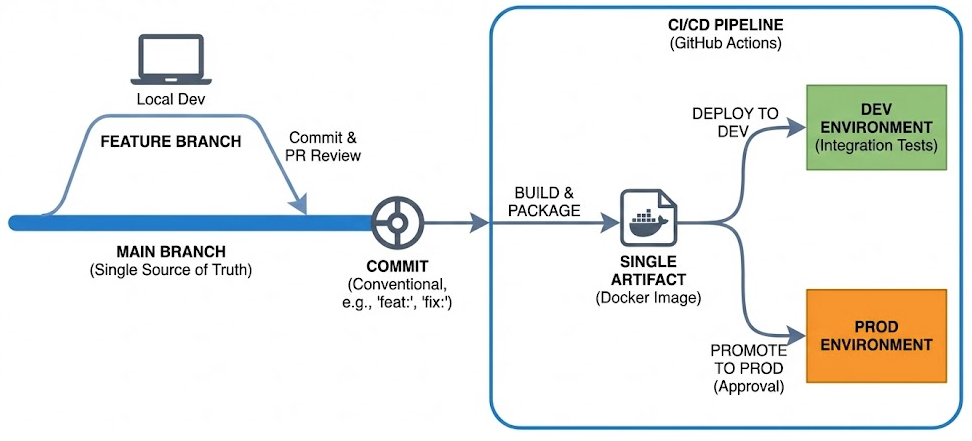
\includegraphics[width=1\textwidth]{images/flusso-commit.png}
    \caption{Flusso architetturale della pipeline CI/CD basata sul Trunk-Based Development. L'unione sul branch principale innesca la generazione dell'artefatto promosso nei vari ambienti [Elaborazione dell'autore].}
    \label{fig:trunk_based_cicd}
\end{figure}

\subsection{Design dell'Interfaccia MCP per l'Automazione Infrastrutturale}

L'adozione rigorosa dell'Infrastructure as Code (IaC) e dei flussi CI/CD basati su GitOps assicura la stabilità e la sicurezza del sistema, ma introduce inevitabilmente una barriera all'ingresso per gli sviluppatori focalizzati unicamente sul dominio applicativo. Per generare un nuovo microservizio, l'operatore è tipicamente tenuto a conoscere la topologia del repository Terraform, le convenzioni di nomenclatura, la sintassi Docker e i costrutti delle pipeline GitHub Actions.

Al fine di mitigare questo sovraccarico cognitivo, la fase di progettazione ha previsto l'ingegnerizzazione di \textit{Service-Forge}, un framework di automazione interno. L'innovazione architetturale risiede nella decisione di non limitare tale strumento a una tradizionale interfaccia a riga di comando (CLI), bensì di esporne le funzionalità attraverso un server conforme al Model Context Protocol (MCP).

Il design prevede che il generatore di microservizi (Service-Forge) agisca come un Server MCP indipendente, sviluppato avvalendosi della libreria Python FastMCP. L'ambiente di sviluppo integrato (IDE) in uso presso l'azienda, dotato di funzionalità di assistenza tramite Large Language Models, funge invece da Client MCP.
Quando uno sviluppatore richiede la creazione di un nuovo servizio fornendo specifiche in linguaggio naturale, l'agente LLM si connette al server FastMCP per ottenere la firma dei metodi disponibili.

\begin{figure}[htbp]
    \centering
    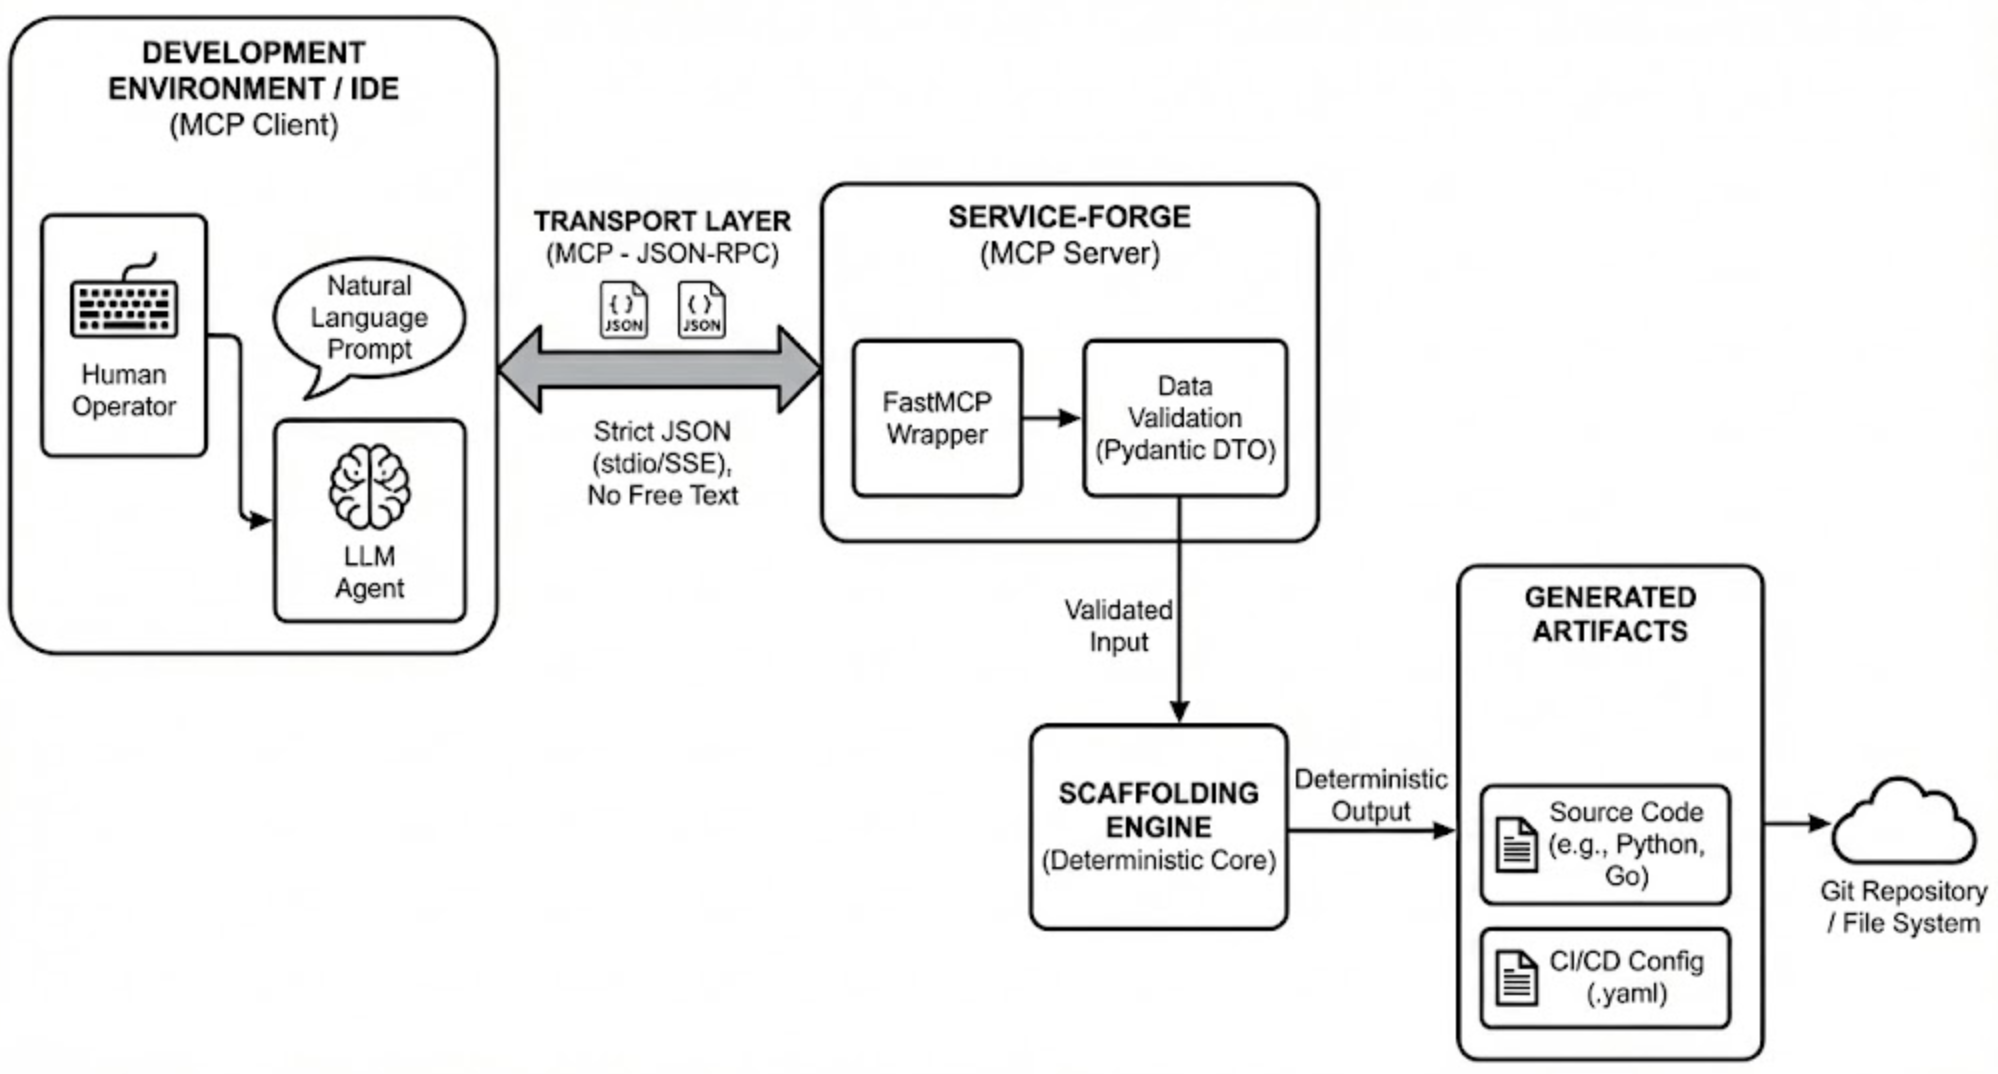
\includegraphics[width=1\textwidth]{images/mcp-architecture.png}
    \caption{Architettura logica dell'integrazione MCP. Il diagramma illustra la separazione delle responsabilità tra l'IDE (Client MCP) delegato all'estrazione semantica tramite LLM, e Service-Forge (Server MCP) responsabile della validazione Pydantic e dell'esecuzione deterministica dello scaffolding [Elaborazione dell'autore].}
    \label{fig:design_mcp_architecture}
\end{figure}

L'architettura delega all'Intelligenza Artificiale esclusivamente l'estrazione semantica dei parametri (es. il nome del servizio, il pattern architetturale desiderato) e la relativa formattazione in una struttura dati JSON valida, come illustrato nello schema di Figura \ref{fig:design_mcp_architecture}. Il nucleo deterministico del sistema (Service-Forge) riceve tale payload, lo sottopone a una rigorosa validazione sintattica tramite schemi Pydantic e, in caso di esito positivo, avvia l'esecuzione del codice di scaffolding.
Questo pattern di progettazione, comunemente noto come AI-Augmented Platform Engineering, confina la non-determinabilità dell'LLM all'interfaccia utente, mantenendo il controllo assoluto e deterministico sulla generazione degli artefatti software e infrastrutturali aziendali.